\documentclass{article}
    \usepackage[UTF8]{ctex}
    \usepackage{caption,amsmath}
    \usepackage{graphicx, subfig}


 \title{ 第三章. 离散数据的生成模型}
 \begin{document}
 \date{}
 \maketitle
 \setcounter{section}{2}
  \section{介绍}
  在2.2.3.2章节中,我们讨论了如何对一个生成式分类器使用贝叶斯规则去分类某个特征向量x
  \numberwithin{equation}{section}
  \begin{equation}
    p(y = c|x,\theta)\propto p(x|y = c,\theta)p(y = c|\theta)
  \end{equation}
  使用这种模型的关键就是为类条件密度指定一个合适的形式$p(y = c|x,\theta)$,适当的形式是指,模型定义了
  我们期望在每个类中看到的数据类型.在本章中,我们集中关注离散数据。
我们还讨论如何推断这些模型的未知参数$\theta$.
   \subsection{贝叶斯概念学习}
   考虑孩子学会如何理解单词的意思,比如“狗”。
   我们可以推测,孩子的父母指出了这个概念的正面例子,
   比如说“看可爱的小狗!”,或者“小心小狗”等等。
   相反,他们提供反面的例子的可能性不大,
   比如他们说“ 看看那只非狗“。 当然,在积极的学习过程中可能会得到负面的例子 - 孩子说“看狗”,父母说“这只猫,亲爱的,而不是狗”
   - 但心理学研究表明,
   人们可以\textbf{只}从正面例子中学习概念(Xu和Tenenbaum,2007)
   \begin{figure}
    \centering
    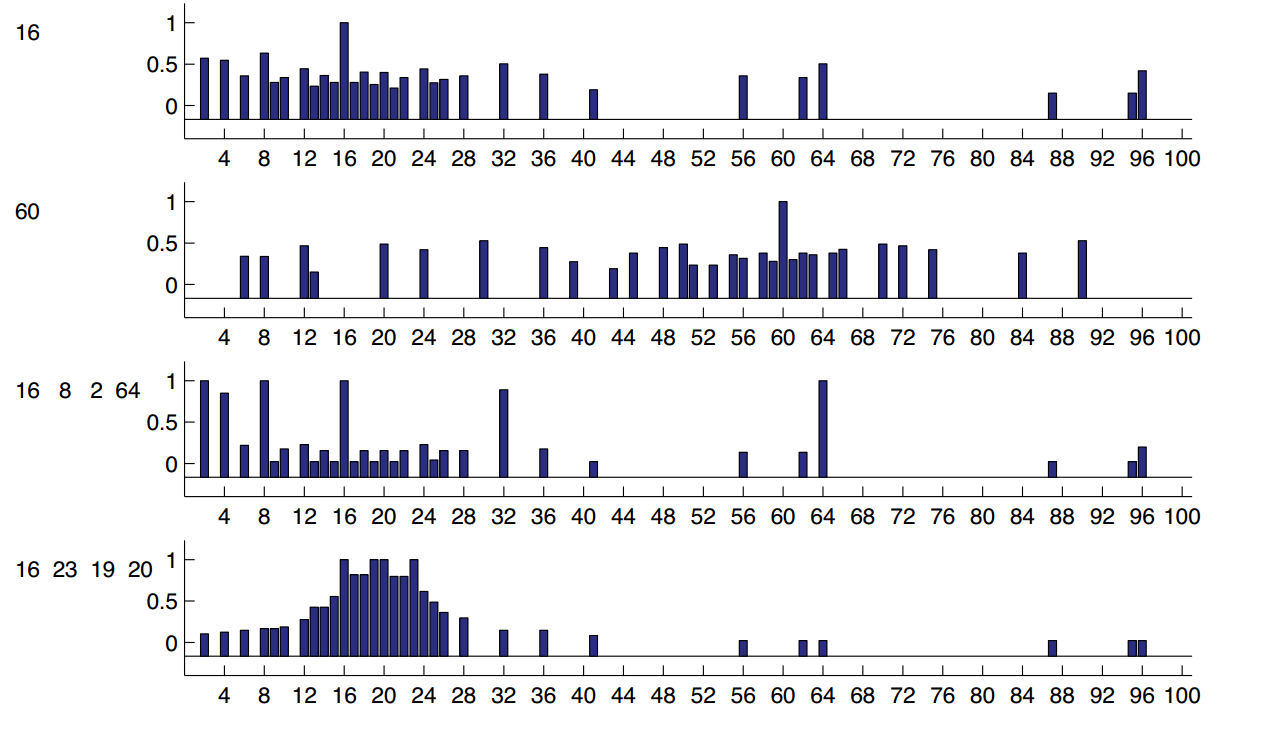
\includegraphics[width=.9\textwidth]{./Picture/31.png} %1.png是图片文件的相对路径
    \caption*{3.1 例子} %caption是图片的标题
    \label{img1} %此处的label相当于一个图片的专属标志,目的是方便上下文的引用
  \end{figure}


\end{document}
